%%%%%%%%%%%%%%%%%%%%%%%%%%%%%%%%%%%%%%%%%%%%%%%%%%%%%%%%%%%%%%%%%%%%%%
%%                     And
%%%%%%%%%%%%%%%%%%%%%%%%%%%%%%%%%%%%%%%%%%%%%%%%%%%%%%%%%%%%%%%%%%%%%%
%\color{blue}
\subsection{Glyph: \glyph{And}}\label{sec:and}

\begin{description}
 \item[SBO]\mbox{}\\ SBO:0000173 ! and.
 \item[origin]\mbox{}\\ More than one EPN (section~\ref{sec:EPNs}) or logical operator (section~\ref{sec:logic}).
 \item[target]\mbox{}\\  Modulation (section~\ref{sec:modulation}), stimulation (section~\ref{sec:stimulation}), catalysis (section~\ref{sec:catalysis}), inhibition (section~\ref{sec:inhibition}) or trigger (section~\ref{sec:trigger}) arcs.
 \item[node]\mbox{}\\ \glyph{and} is represented by a circle carrying the word ``AND''.
 \end{description}

\begin{figure}[H]
  \centering
  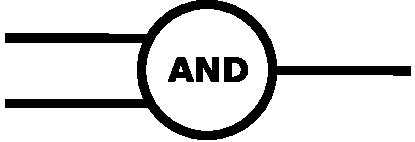
\includegraphics[scale = 0.5]{images/and}
  \caption{The \PD glyph for \glyph{and}.}
  \label{fig:and}
\end{figure}


% The following diagrams illustrate the dephosphorylation of the MAP inase ERK by the protein phosphatase 2A and the STriatal Enriched Phosphatase, in ST (left) and ER (right). 
% 
% \begin{center}
% \scalebox{0.5}{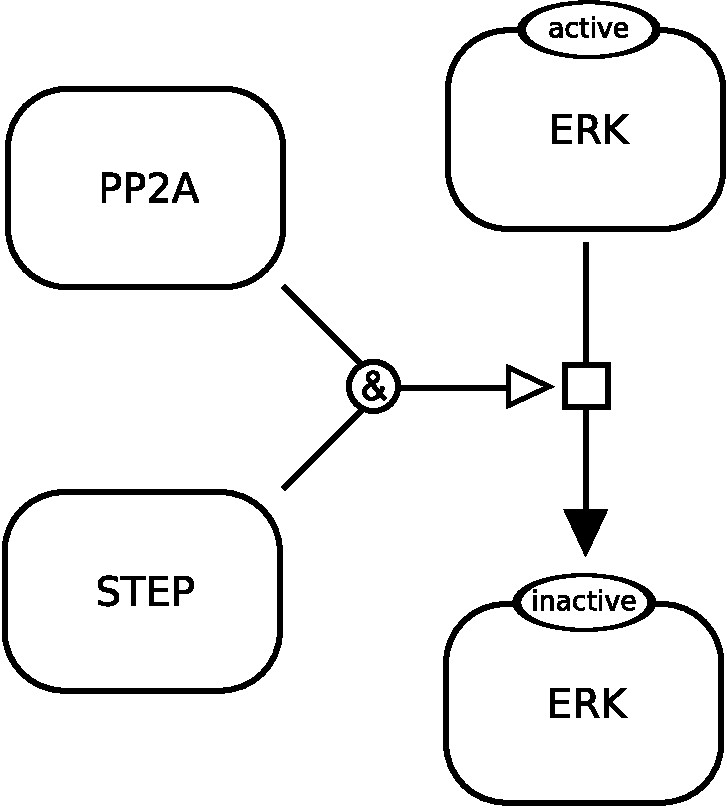
\includegraphics{images/stimulation-example1}}
% \end{center}
\normalcolor
